\section{Evaluation}
\label{sec:eval}
We measured our DNS rebinding attack by two primary factors. We analyzed the \emph{time to launch} and the \emph{impact} of the attack. We then compared it to other two DNS rebinding mechanisms. 

\subsection{Time to Launch}
To protect from a time-varying attack that is able to establish an interactive session between the malicious server and the broswer, most modern browers have implemented DNS pinning that pin a DNS record for a period of time. At this time, a time-varying attack would take ~160 seconds to launch according to our experiment on the latest Chrome browser. However, by flooding the DNS table, we found that in the current Chrome implementation, if a DNS record is kicked out from the cache, the pinning time would dramatically decrease. We found that in our attack, only ~10 seconds is needed to launch the attack on a browser that have 100 entries. 

In early 2013, the Chromium community has increased the size of DNS cache from 100 to 1000. This is not a really security patch but a performance related patch. We then ran our experiments on the staging version Chrome, and found that it would only take 10 more seconds to flood the DNS table and launch the attack. 

Another approach of DNS rebinding is based on multiple A records attack. This attack needs only a small amount of time due to the number of packets transmitted, however this attack has certain limitations, we will discuss it in the next subsection.

\subsection{Impact}
We now evaluate the impact of our attack against other DNS rebinding approaches. As mentioned in the last section, the multiple DNS record approach has the advantage of using less time to launch. However, it has several limitations on its impacts. 1) The rebinded IP address cannot be an internal IP address, otherwise the browser will priorize it and select it in the first place which results in a failure in DNS rebinding. 2) The attacker cannot change the rebinded IP address on the fly, which makes it unable to scan the subnet. 

For time-varying attack, although it is possible to bind to an internal IP address, it is also hard to change the rebinded IP address on the fly due to the extremly long launching time. 

In our experiement, we are able to use FireDrill to rebind the domain name to an internal IP address to build a interactive session. Also, we are able to dynamically change the IP address during an attack. The attacker has the ability to navigate through the entire subnet instead of just one single IP address.

\subsection{Making The Victim Stay}
Our attack needs the victim's browser to act as a proxy. Thus it requires the victim to stay in the page for the attacker to have access to it. In order to do that, we designed a ``pending download`` page \ref{fig:download} that ask the victim to stay in the page for two minutes to download a file. While the victim is waiting for the download countdown, the Javascript proxy is actually running in the background for the attacker to navigate through the internal websites.

\begin{figure}[h]
\centering

\includegraphics[width=0.8\columnwidth]{download.png}
\caption{The download page that a victim is first connecting to. While waiting for the file to be downloaded, the javascript is running in the the background as a proxy.}
\label{fig:download}
\end{figure}

\subsection{Changing the Content of Internal Wiki}
Now we demonstrate how to use FireDrill to access a victim's internal wiki. 

Reference the figure like this: Figure \ref{fig:oldrevisions}.
\begin{figure}[h]
\centering
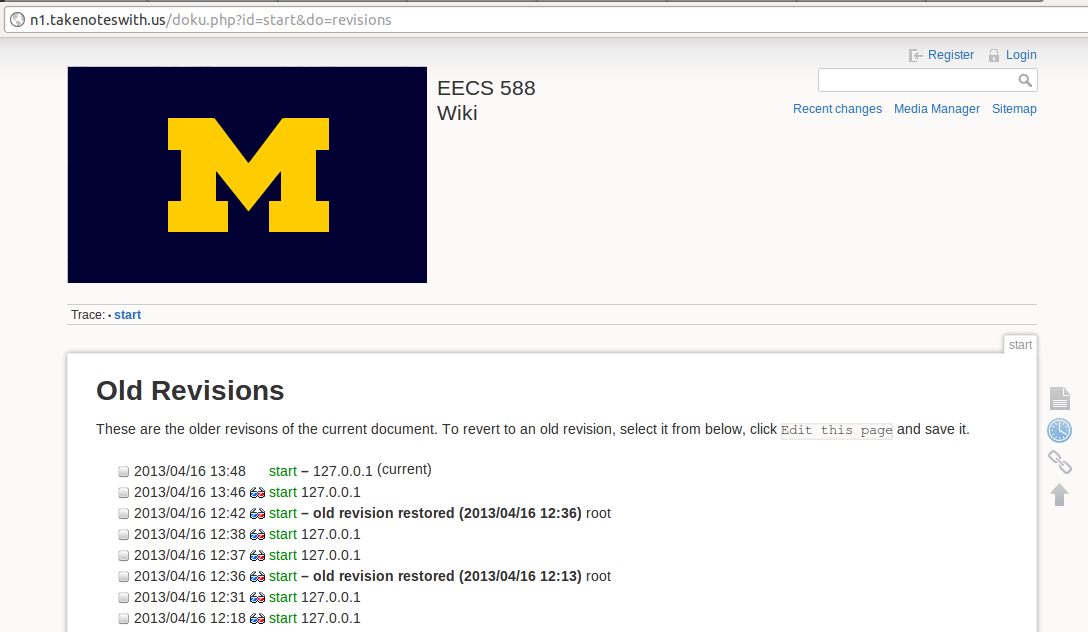
\includegraphics[width=0.8\columnwidth]{oldrevisions.png}
\caption{\textbf{xyz.} xyz}
\label{fig:oldrevisions}
\end{figure}

